This chapter contains documentation about the implementation of the protocol designed in Chapter \ref{cha:protocolDesign}. 

First, the classes used in the implementation are shown and explained. Then important parts of the sourcecode are explained.
 

\section{General}
The implementation is written in C++. The development of the solution is done in two man teams, using pair programming. Git is used for version control. The implementation is designed with the requirements of the solution along with the components and choices made in Chapter \ref{cha:designintro}. 

Note that the code in the listings does not necessarily contain the same comments and print statements as in the actual code, to make the code fit onto the pages in the report.

\section{Classes}
The solution contains two different running applications. The main node and the sensor nodes. There are two sets of code due to the different requirements of the nodes. For example, the main node does not have a sensor, as explained in Chapter \ref{cha:workflowDesign}, so it should not be able to handle a sensor, and therefore does not contain the classes used for sensors.

This section contains the classes contained in each application. UML diagrams showing all fields and methods for both main and sensor nodes can be found in Appendix \ref{cha:fulluml}.

\subsubsection*{Main node}
The main node is a Raspberry Pi device, running the Raspbian operating system. The classes in the main node application is seen in figure \ref{fig:mainnodeClass}. 
According to the specification, the main node pairs nodes, sends requests, and handles received data.

\begin{figure}[h!]
\centering
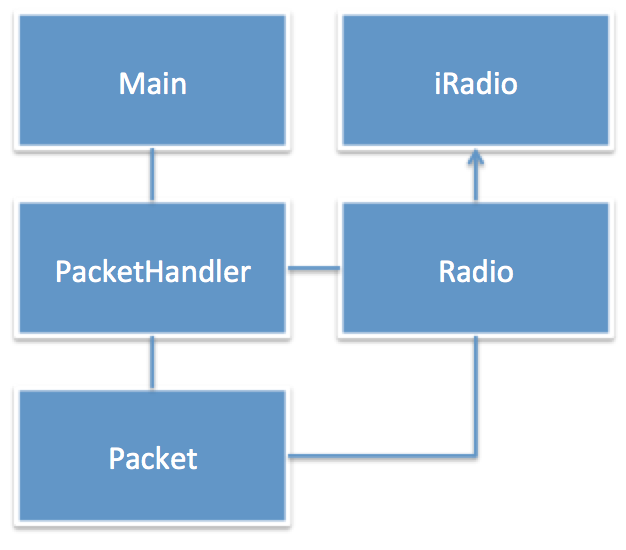
\includegraphics[width=0.65\textwidth]{chapters/implementation/figures/mainnodeClass.png}
\caption{Classes used in the main node.}
\label{fig:mainnodeClass}
\end{figure}



\subsubsection*{Sensor nodes}
The platforms used for the sensor nodes are Arduino Uno and Mega, although one platform per node. The differences between the two platforms are the pins used for the sensor and radio modules. Besides the pin number, the code is identical on the two platform types. 

The classes used in the nodes are seen in figure \ref{fig:nodeClass}.
\begin{figure}[h!]
\centering
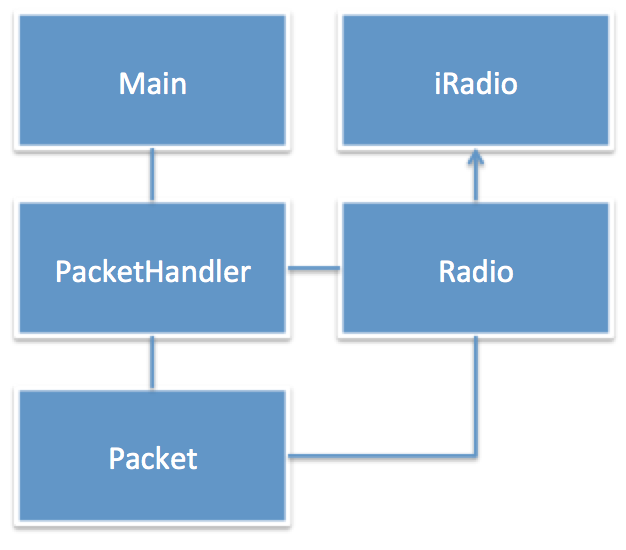
\includegraphics[width=0.85\textwidth]{chapters/implementation/figures/nodeClass.png}
\caption{Classes used in nodes.}
\label{fig:nodeClass}
\end{figure}


\subsubsection*{Class descriptions}
This section contains explanations about the classes used in the nodes. As the classes are reused on both main and sensor nodes they are only explained once, even though the code may be somewhat different.

\begin{description}
\item[Node] \hfill \\
The \texttt{Node} class is the entry point in the application.
On the sensor node, it contains one or more \texttt{iSensor}s, and a \texttt{iRadio} object that are instantiated when the code is run. The main node contains no sensor, but an \texttt{iRadio} object exists.

The \texttt{Node} class determines what action to take when a packet is received. If data is received from another sensor node that should be relayed, the \texttt{Node} begins sending data until an acknowledgment is received. The methods on the \texttt{iRadio} object is used for listening and sending.
If data is needed for a packet, for example when a request is received, the \texttt{Node} class fetches data from the sensor, and creates the packet that needs to be sent, and makes sure that the data is sent.

\item[iRadio and iSensor] \hfill \\
The \texttt{iSensor} and \texttt{iRadio} interfaces are used to establish a way that all sensors and radio module classes should work. This means that replacing or adding a new sensor or using another radio module is possible, as long as the new component adheres to one of these interfaces. This makes the rest of the code know how to use these components. 

\texttt{iSensor} only contains the method \texttt{int read()}, that returns the value of the sensor. Sensors can contain different methods internally to verify or handle data, but will be required to have the \texttt{read} method.

\texttt{iRadio} contains the methods needed for receiving and sending packets. A special listen method is needed for implementing exponential backoff as the listen function blocks execution and a way of breaking this blocking is needed to not lock the code.
\begin{description}
\item[void broadcast(char *packet)] sends a packet
\item[char *beginListening()] begins listening
\item[char *listenFor(int ms)] begins listening, but stops listening after 'ms' ms
\end{description}

\item[Sensor] \hfill \\
The \texttt{Sensor} class can be used for multiple sensors, as long as the sensor class inherits from \texttt{iSensor}. This class' job is to read data from a sensor on the node, handle this data, and return it to the class that requested this data.

In the solution the sensor class is called \texttt{MoistureSensor}, as a moisture sensor is used. This class can only be found on the sensor nodes, and not on the main node.


\item[NRF24Radio] \hfill \\
The \texttt{NRF24Radio} class handles the radio communication. Classes of this class should inherit from the \texttt{iRadio} interface as the application uses this interface to handle all radiocommunication. The \texttt{NRF24Radio} class returns a \texttt{char} pointer when a packet is received, using one of the listening methods explained in the \texttt{iRadio} section. It is also able to send packets given from other classes, using the \texttt{broadcast} method.

\item[Packet] \hfill \\
The class \texttt{Packet} has the ability to parse a packet from a \texttt{char} array to a \texttt{Packet} object, along with the properties required to further handle the packet. This includes the type, and possibly sensor values, sender and receiver values or an identifier from the main node.

Instances of this class is created and used in the \texttt{Node} class. The objects are created when the radio returns the \texttt{char} array from the listen methods. The packet is then used before it is freed.

This class contains the public methods:
\begin{description}
\item[Packet(char *input)] Create a packet from a char array. Used when radio receives a packet.
\item[{\parbox[t]{0.6\linewidth}{Packet(PacketType packetTypeInput, \\ uint16\_t addresserInput, \\ uint16\_t addresseeInput, \\ uint16\_t originInput, \\ uint16\_t value1Input, \\ uint16\_t value2Input, \\ uint16\_t value3Input)}}] \item[] Creates a new packet with data as noted in parameters.
\item[char *encode()] Returns a char array representation of the packet. Used for broadcasting from the radio.
\end{description}

\end{description}


\section{Code}\todo{AAAAHHH!!!!! single lines!?!}
This section contains explanations for some of the important parts of the code.

First, the \texttt{Packet} implementation is explained, with code showing how values are handled and how CRC is implemented.

Second, the \texttt{Node} class is explained along with sensor nodes.

Last, the main node and its interface is explained.

\subsection{Packet}
The \texttt{Packet} class contains the data from a packet received from the radio module. It can be instantiated with a string, or with every part of the packet as a parameter, using the constructors in Listing \ref{lst:packetconstructors}.
\begin{lstlisting}[language=C,label={lst:packetconstructors},caption={Packet constructors}]
Packet::Packet(PacketType packetTypeInput, uint16_t addresserInput, uint16_t addresseeInput, uint16_t originInput, uint16_t value1Input,
	uint16_t value2Input, uint16_t value3Input)
	
Packet::Packet(char *input)
\end{lstlisting}


This class is passed around in \texttt{Node}, where it is used to determine actions based on the type, or being relayed with some new data. 
The class itself contains the variables:
\begin{figure}
\begin{lstlisting}
PacketType packetType; // The type of the packet
uint16_t addresser; // The sender of the packet (node ID)
uint16_t addressee; // The receiver of the packet (node ID)
uint16_t origin; // The original sender of the packet
uint16_t value1; // Value 1 (Used for sensor value)
uint16_t value2; // Value 2
uint16_t value3; // Value 3
uint16_t checksum; // Checksum value
\end{lstlisting}
\end{figure}
These values cover everything in a packet; the type, the sender, the receiver, the origin of the packet, values and a checksum.
Every packet has this format, and all values are filled out. With packets that might not require all these values, they will simply be zero. For example when sending a request, the sensor values and addressee will be zero.

\begin{table}[]
\centering
\begin{tabular}{|l|c|l|c|l|c|l|c|l|}
\hline
\textbf{Datatype} & \multicolumn{2}{c|}{Packettype}      & \multicolumn{2}{c|}{uint16\_t}       & \multicolumn{2}{c|}{uint16\_t}       & \multicolumn{2}{c|}{uint16\_t}       \\ \hline
\textbf{Name}     & \multicolumn{2}{c|}{packetType}      & \multicolumn{2}{c|}{addresser}       & \multicolumn{2}{c|}{addressee}       & \multicolumn{2}{c|}{origin}          \\ \hline
\textbf{Memory}   & \multicolumn{1}{l|}{8 bits} & 8 bits & \multicolumn{1}{l|}{8 bits} & 8 bits & \multicolumn{1}{l|}{8 bits} & 8 bits & \multicolumn{1}{l|}{8 bits} & 8 bits \\ \hline
\end{tabular}
\caption{Overview of first half of a packet. The packet can be directly converted to 16 characters.}
\label{tab:packetTableFirst}
\end{table}

\begin{table}[]
\centering
\begin{tabular}{|l|c|l|c|l|c|l|c|l|}
\hline
\textbf{Datatype} & \multicolumn{2}{c|}{uint16\_t}       & \multicolumn{2}{c|}{uint16\_t}       & \multicolumn{2}{l|}{uint16\_t} & \multicolumn{2}{c|}{uint16\_t}       \\ \hline
\textbf{Name}     & \multicolumn{2}{c|}{value1}         & \multicolumn{2}{c|}{value2}         & \multicolumn{2}{c|}{value3}   & \multicolumn{2}{c|}{checksum}        \\ \hline
\textbf{Memory}   & \multicolumn{1}{l|}{8 bits} & 8 bits & \multicolumn{1}{l|}{8 bits} & 8 bits & 8 bits         & 8 bits        & \multicolumn{1}{l|}{8 bits} & 8 bits \\ \hline
\end{tabular}
\caption{Overview of second half of a packet.}
\label{tab:packetTableSecond}
\end{table}

The datatype of the members of \texttt{Packet} are all \texttt{uint16\_t}. This is to ensure that the size of the class does not vary on different architectures. The \texttt{uint16\_t} is always of size 2 bytes. The same size as two characters. Together, all members in the class gives a total size of 16 bytes. The final architecture of a packet can be seen on \ref{tab:packetTableFirst} and \ref{tab:packetTableSecond}.

Only half of the space available in a transmission are occupied as the radio module used in this project supports transmissions of 32 byte at a time. As the solution is designed modular, and the radio module can be replaced with a potentially 'smaller' module in terms of transmission size, the solution would still support this 'smaller' module. Furthermore, a packetsize of 16 bytes is enough to contain the different data collected from the nodes.

\texttt{PacketType} is defined as follows:
\begin{lstlisting}[language=C]
enum PacketType : uint16_t {
    Error,
    DataAcknowledgement,
    DataRequest,
    Data,
    PairRequest,
    PairRequestAcknowledgement,
    ClearSignal
};
\end{lstlisting}


When a \texttt{Packet} is instantiated using the constructor with the \texttt{char *input} as parameter, these values are found using the function \texttt{memcpy}, in the \texttt{decode} function, seen in Listing \ref{lst:decodefunc}.
\begin{lstlisting}[language=C,label={lst:decodefunc},caption={Decode function.}]
void Packet::decode(char *input)
{
    memcpy(this, input, sizeof(Packet));
}
\end{lstlisting}
This copies the memory of the \texttt{char *input} into the memory location where the current \texttt{Packet} object is located. This means that the contents of the packet is set to the content of \texttt{input}.

This is possible as every part of the packet has a known, pre-determined size. \texttt{uint16\_t} always has the same size, not dependant on the architecture running the code. When a packet is encoded, using the \texttt{char *encode()} function, the returned character array is built in the same way, by setting the contents of the array to the contents of the package.

\begin{lstlisting}[language=C]
char *Packet::encode()
{
    char *returnstring;
    returnstring = (char*)malloc(sizeof(Packet));

    memcpy(returnstring, this, sizeof(Packet));

    return returnstring;
}
\end{lstlisting}
The \texttt{encode} function allocates the size necessary for a \texttt{Packet}, but as a \texttt{char *} and uses \texttt{memcpy} to set the contents of the array to the contents of the current \texttt{Packet} and then returning the array. The char array can be seen as a format of the packet object, that can be directly transmitted by the radio module without further operations to the array.

\subsubsection{Checksum}
\texttt{Packet} objects contains a checksum, used to verify the content's integrity. The checksum uses two functions: \texttt{crcInit()} and \texttt{crcCompute(unsigned char *message, unsigned int nBytes)}. The checksum implementation is based on the description in \texttt{Programming Embedded Systems in C and C++} \cite{crcCode}.

The CRC functions share the following data, and this data should be implemented so that it is usable by the functions without instantiating them multiple times and use more memory than necessary.

\begin{description}
	\item[POLYNOMIAL] the generator polynomial by which the message is divided.
	\item[INITIAL\_REMAINDER] the remainder initially appended onto the message before calculating the checksum.
	\item[FINAL\_XOR\_VALUE] the value by which the transfer message is inverted.
	\item[WIDTH] the width of the checksum, which in CRC-16 is 16 bits.
	\item[TOPBIT] is the most significant bit set to 1.
\end{description}

The \texttt{crcInit()} should be run initially to instantiate a table of remainders to expedite the computation of the checksum. The computation is accelerated because the remainder can be calculated byte-wise instead of bit-wise, by the cost of 256 bytes in the memory.  

\begin{lstlisting}[language=C]
void Packet::crcInit()
{
    unsigned short remainder; // 2 byte remainder (according to CRC16/CCITT standard)
    unsigned short dividend;  // What are you?
    int bit; // bit counter

    for(dividend = 0; dividend < 256; dividend++) //foreach value of 2 bytes/8 bits
    {
        remainder = dividend << (WIDTH - 8);//

        for(bit = 0; bit < 8; bit++)
        {
            if(remainder & TOPBIT) // MSB = 1 => divide by POLYNOMIAL
            {
                remainder = (remainder << 1) ^ POLYNOMIAL; //scooch and divide
            }
            else
            {
		        remainder = remainder << 1;//scooch and do nothing (MSB = 0, move along)
	        }
        }
    	Packet::crcTable[dividend] = remainder;//save current crc value in crcTable
    }
}
\end{lstlisting}

The function iterates over all binary combinations of the 16 bits for the dividend. Within this iteration each remainder is initially instantiated by shifting the dividend by 8 bits, as the purpose is to generate 1 byte values. For each of the 8 bits, if the remainders most significant bit is 1, the remainder is divided by the \texttt{POLYNOMIAL} and left shifted one bit. If the most significant bit is 0, the remainder is only left shifted one bit. When all 8 bit computations are finished, the remainder is saved to the \texttt{crcTable} in the current \texttt{dividend}'s position.

However, the main CRC function is the \texttt{getChecksum(unsigned char *message, unsigned int nBytes)}. It utilizes the \texttt{crcTable} and computes and returns the transfer message based on the arguments \texttt{unsigned char *message} and the size of the message \texttt{unsigned int nBytes}.

\begin{lstlisting}[language=C]
uint16_t Packet::getChecksum(unsigned char *message, unsigned int nBytes)
{
    unsigned int offset;
    unsigned char byte;
    uint16_t remainder = INITIAL_REMAINDER;

    for (offset = 0; offset < nBytes; offset++)
    {
        byte = (remainder >> (WIDTH - 8)) ^ message[offset];
        remainder = Node::crcTable[byte] ^ (remainder << 8);
    }
    uint16_t result = remainder ^ FINAL_XOR_VALUE;

    char *toBeSwapped = (char*)malloc(sizeof(char)*2);
    memcpy(toBeSwapped, (char*)&result, sizeof(char)*2);
    char temp = toBeSwapped[1];
    toBeSwapped[1] = toBeSwapped[0];
    toBeSwapped[0] = temp;

    memcpy((char*)&result, toBeSwapped, sizeof(char) * 2);
    free(toBeSwapped);
    return result;
}
\end{lstlisting}


\texttt{getChecksum} uses an \texttt{int offset} to keep track of the iterative progress through the message, a \texttt{char byte} to contain a byte of the \texttt{message} and a \texttt{uint16\_t remainder} instantiated by the \texttt{INITIAL\_REMAINDER} value. 

The function iterates over each byte in the \texttt{message}, according to the algorithm described in Section \ref{cha:crcComp}. The current \texttt{byte} is the remainder right shifted by 8 then XOR'ed with the \texttt{message}'s offset byte. The \texttt{remainder} is then calculated by XOR'ing the value already stored in \texttt{crcTable} at the current byte, with the remainder left shifted by 8. \todo{review explanation}
\subsection{Node}
The \texttt{Node} class is used as a static class, which means that only one instance of it exists. This class determines the action to take when a packet is received, which takes place in the function \texttt{void handlePacket(Packet packet)}, where a \texttt{switch} statement is used based on the packet type.

\texttt{Node} also makes sure that packets are transferrered correctly. This means sending packets until an acknowledgement or other confirmation has arrived. To ensure this, exponential backoff is used, as explained in Chapter \ref{cha:expbackoff}.

The implementation of the \texttt{Node} classes are different on the main node and sensor nodes, which are explained in the following two sections.

\subsection{Sensor nodes} 


\subsection{Main node} \label{cha:signalhandling}
The main nodes tasks are to request and receive values from nodes. Once the values are received, they are saved, until all nodes have been accounted for, or a timeout is hit.

When the request is done, the data is saved to a file with the name of the current date and time. Another file is also saved, which is used for knowing when the request is done in the webinterface, as explained in Chapter \ref{cha:webinterface}. The request is started when a signal of the type \texttt{SIGUSR1} is received. This sets a flag, \texttt{signalReceived} in \texttt{Node} to 1. The next time the main loop is run, the request will be send, and the flag set to 0 again.
\subsection{User interface} \label{cha:webinterface}
Users of the system has to be able to start a request and to see data from the nodes when the request is complete. To make this possible, a user interface was developed, that allows users to start requests and see data from this and previous requests.

The interface runs as its own program, as a CGI (Common Gateway Interface) program running on the Raspberry Pi device, using Apache. The executable is located in \texttt{/usr/lib/cgi-bin/} and is called \texttt{WASP}. The program is written in C, and the complete code can be found in appendix \ref{cha:uicode}.

When this program is executed, it prints out HTML. Because it is executed as a CGI program using Apache, it is possible to connect to this program using a browser. When connected to the 'website', the user is able to make requests or show previous results. When a link is clicked, a string is appended onto the current URL, for example \texttt{?request}. The string after the '?' is passed as an argument to the script.

On startup, the program attempts to fetch the process ID of the main node program, located in \texttt{/var/run/} if the program is running. This PID is used when the request button is presed by the user. The PID is necessary to call the procedure \texttt{kill}, that is used to signal the main node software that it should start a request. The signal is handled as explained in chapter \ref{cha:signalhandling}. Kill is a function that sends a signal to one or many processes. In the solution, the signal \texttt{SIGUSR1} is used.

When \texttt{kill} is issued, the program redirects to a waiting page. On this page, an AJAX request is performed every second to ping for a file in \texttt{/var/www/html/}. This ping will fail until the file \texttt{ping.txt} exists at this location. When the request is finished in the main node software, this file is created and the contents is set to the result name. When the file is written and closed by the main node software, the ping will succeed and the contents will be available. The browser can now be redirected to the result from the waiting screen. The ping file is then deleted as it is no longer needed.

The full sequence is shown in figure \ref{fig:sigsequence}. The diagram starts at the webinterface, and the sequence follows the numbers presented on the diagram.
\begin{figure}[h!]
\centering
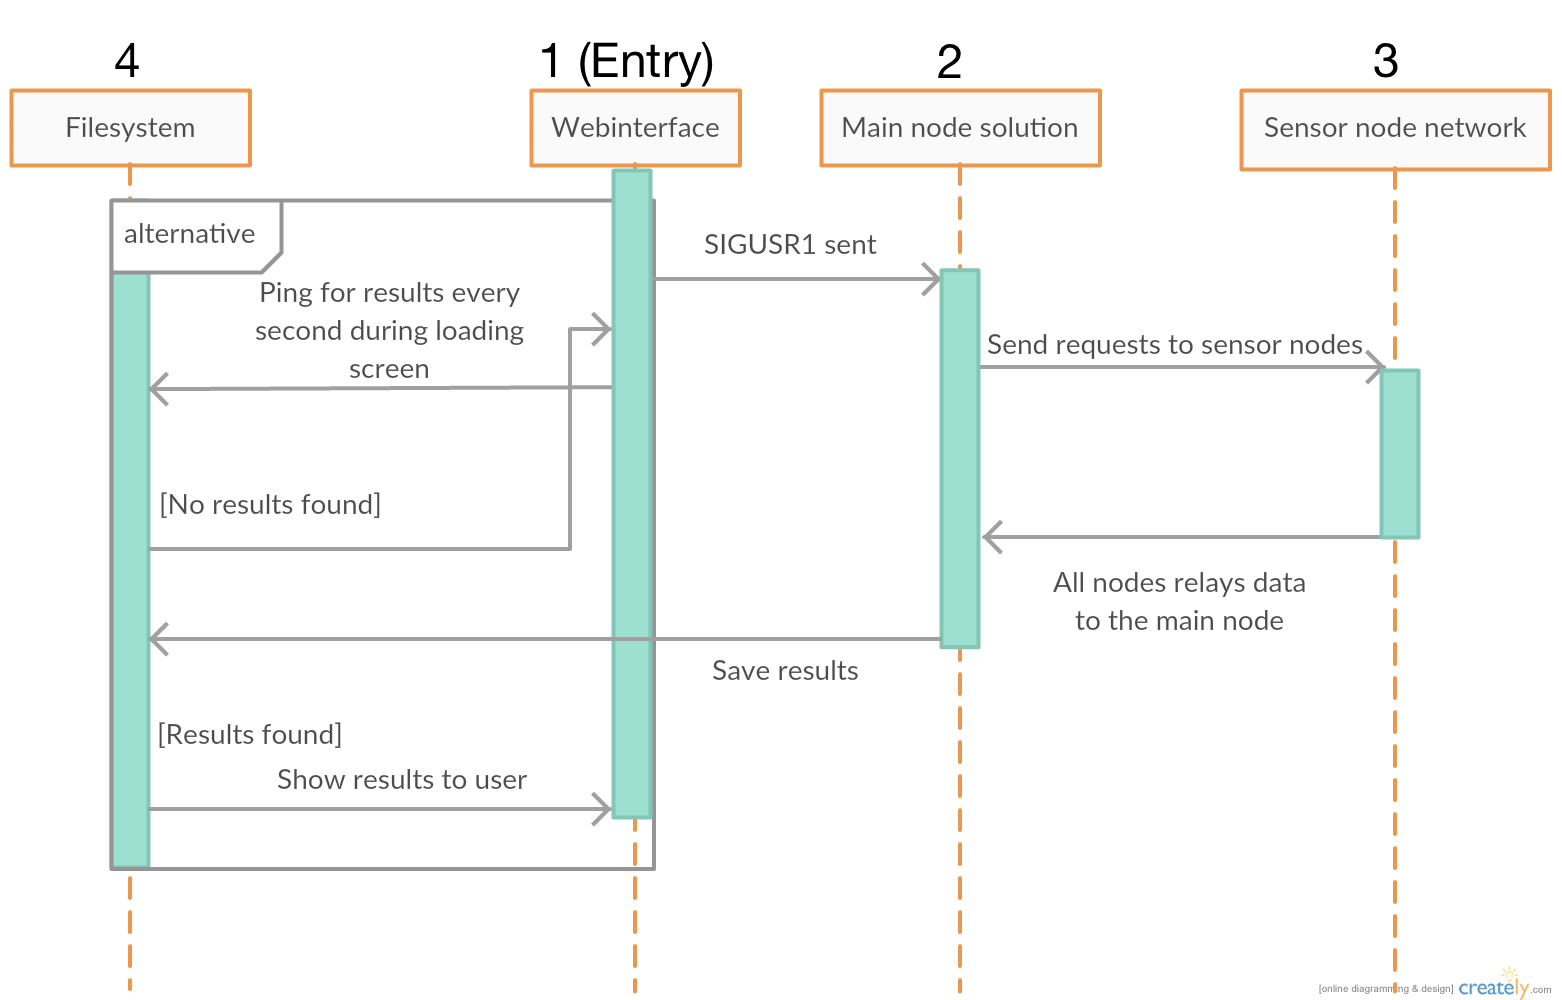
\includegraphics[width=1.1\textwidth]{chapters/implementation/figures/sigsequence.png}
\caption{Full sequence from webinterface to results\cite{creately}.}
\label{fig:sigsequence}
\end{figure}